\documentclass[12pt,a4paper]{article}

\usepackage[caption=false,font=normalsize,labelfont=sf,textfont=sf]{subfig}
\usepackage{times}
\usepackage{indentfirst}
\usepackage{amssymb}
\usepackage{color}
\usepackage{graphicx}
\usepackage{url}
\usepackage{float}
\usepackage{stfloats}
\usepackage{rotating}
\usepackage{listings}
\usepackage{xcolor}
\usepackage{color}
\usepackage{tabularray}
\usepackage{bbding}
\newtheorem{theorem}{Theorem}
\newtheorem{acknowledgement}[theorem]{Acknowledgement}
\newtheorem{algorithm}[theorem]{Algorithm}
\newtheorem{axiom}[theorem]{Axiom}
\newtheorem{case}[theorem]{Case}
\newtheorem{claim}[theorem]{Claim}
\newtheorem{conclusion}[theorem]{Conclusion}
\newtheorem{condition}[theorem]{Condition}
\newtheorem{conjecture}[theorem]{Conjecture}
\newtheorem{corollary}[theorem]{Corollary}
\newtheorem{criterion}[theorem]{Criterion} 
\newtheorem{definition}[theorem]{Definition}
\newtheorem{example}[theorem]{Example}
\newtheorem{exercise}[theorem]{Exercise}
\newtheorem{lemma}[theorem]{Lemma}
\newtheorem{notation}[theorem]{Notation}    
\newtheorem{problem}[theorem]{Problem}
\newtheorem{proposition}[theorem]{Proposition}
\newtheorem{remark}[theorem]{Remark} 
\newtheorem{solution}[theorem]{Solution}
\newtheorem{summary}[theorem]{Summary}
\newenvironment{proof}[1][Proof]{\noindent\textbf{#1.} }{\ \rule{0.5em}{0.5em}}
\setlength\textwidth{6.5in}
\setlength\textheight{9.0in}
\setlength\oddsidemargin{0.0in}
\setlength\evensidemargin{0.0in}
\setlength\topmargin{-0.5in}
\usepackage{amsmath,amssymb}
\usepackage{mathtools}
\usepackage{amsfonts}
\usepackage{xcolor}
\usepackage{algorithm}
\usepackage{algpseudocode}
\usepackage{textcomp,booktabs}
% \usepackage[table,xcdraw]{xcolor}
\usepackage{makecell}
\usepackage{wrapfig}
\usepackage{multirow}
\usepackage{colortbl,booktabs}
\usepackage{verbatim}
\usepackage[colorlinks,linkcolor=blue]{hyperref}
% \input{tcilatex}
\usepackage{caption}
\usepackage{hyperref}

\newcommand{\C}[1]{{\cal {#1}}}
\usepackage[top=2.5cm, bottom=2.5cm, left=2.5cm, right=2.5cm]{geometry}

% 定义一个名为 \revised 的宏,该宏接受一个参数,即要设置颜色的文本内容
\newcommand{\revised}[1]{\textcolor{cyan}{#1}}
\newcommand{\revisedred}[1]{\textbf{\textcolor{red}{#1}}}

\topmargin -0.05in

\begin{document}

\hspace{4in}%


\bigskip

\hspace{-\parindent}%

\noindent Dear Professor Han-Wei Shen (Editor-in-Chief of TVCG), the Associate Editor, and All Reviewers,

\bigskip

Enclosed please find the newly-improved version of our paper entitled “\textbf{\textit{A Unified Particle-Based Solver for non-Newtonian Behaviors Simulation}}” .  According to all the reviewers’ comments and suggestions, we have revised our manuscript (ID: TVCG-2023-09-0590) and addressed all the reviewers' comments in this revised manuscript. We have re-submitted it to the manuscript central for your examination.
\vspace{0.5cm}

%The reviewers agreed on the technical merits of our work, and the meta reviews raised concerns regarding: 1) Add missing references as suggested by the reviewers; 2) Fix typographical and grammatical errors; 3) Clarify which Generalized Maxwell Model (GMM) is used as requested by reviewer 2; 4) Carefully read all reviews and also address the other comments of the reviewers.

We wish to extend our gratitude to all four reviewers for their detailed comments and insightful suggestions.
In response to the Assosicate Editor's and reviewers’ comments, we have thoroughly revised our manuscript to address all the suggestions and comments. Meanwhile, we mark our modified text in blue in the revised manuscript attached at the end of the response letter to highlight our revisions. %The improvements to our revised manuscript include:

%\begin{itemize}
%    \item We have added all missing references as suggested by the reviewers.
%    \item We have fixed the typographical and grammatical errors pointed out by the reviewers, and improved the writing issues of the entire manuscript as best as we can.
%    \item We have supplemented the related description of the GMM model.
 %   \item We have carefully addressed all the other comments and made corresponding modification in our revised manuscript.
%\end{itemize}
\vspace{0.5cm}
We sincerely appreciate the patience of the editorial team during this process. We hope that our efforts to improve the quality of the paper are evident in the revised manuscript. We would like to express our sincere gratitude for the reviewers’ efforts and time devoted to the manuscript, as well as the constructive feedback. It is our sincere hope that this version is satisfactory and that the paper will get your final acceptance. If you have further concerns, please let us know at your earliest convenience (via qin@cs.stonybrook.edu). 


\bigskip

\noindent Best Regards,


\bigskip

\noindent The authors

\bigskip
\bigskip
\bigskip

\newpage


%=============================================================================
%Responses to the Comments of the Editor
%=============================================================================

\newsavebox\CBox
\def\textBF#1{\sbox\CBox{#1}\resizebox{\wd\CBox}{\ht\CBox}{\textbf{#1}}}
\title{\Large\textbf{ Responses and the Detailed Description of Changes}}
\date{}
\author{}
\maketitle

%==============================================================================
\vspace{-1.5cm}
\begin{flushleft}
	\textit{\textbf{Responses to the Comments from the Associate Editor}}
\end{flushleft}

%==============================================================================

\vspace{0.4cm}
\noindent$\bullet$ \enspace \textbf{Comment:}
\textit{The reviewers agree that the paper is well written and addesses an interesting topic in computer graphics. Please address their remaining comments in a minor revision:\\
- Add missing references as suggested by the reviewers.\\
- Fix typographical and grammatical errors.\\
- Clarify which Generalized Maxwell Model (GMM) is used as requested by reviewer 2.\\
- Carefully read all reviews and also address the other comments of the reviewers.}

\vspace{0.2cm}
\textbf{Response:}
Thank you very much for your kind and favorable consideration on our submission. In response to the feedback from all reviewers, we have made the following modifications: 

1) We have included all missing references as recommended by the reviewers; 

2) We have corrected the typographical and grammatical errors as best as we can; 

3) We have augmented the description of our GMM model and clarified that it is an adapted model, to facilitate a better understanding for readers;

4) We have detailed addressed each of the reviewers' comments. For clarity, we also attached a revised version of manuscript to help track the change easily, where marked the modified text in blue to denote the improvements.

\vspace{0.5cm}
We appreciate your assistance and kind help with our manuscript. We hope our revised manuscript is satisfactory and we can receive your final acceptance.

% ------------------------------------------------------------------
%                                  reviewer1                                   %
% ------------------------------------------------------------------
\newpage
\vspace{-1.5cm}
\begin{flushleft}
	\textit{\textbf{Responses to the Comments from Reviewer 1}}
\end{flushleft}

% ----------------------------- reviewer 1 comment 1 ---------------------------- %

\vspace{0.4cm}
\noindent$\bullet$ \enspace \textbf{Comment 1:}
\textit{The paper needs editing as there are many typographical and grammatical errors. I will mention a few below, but there are many more. }

\vspace{0.2cm}
\textbf{Response:}
Thank you for your meticulous review, and we apologize for the oversights in our manuscript. We have corrected these typographical errors and conducted a thorough check throughout the document to the best of our ability.

% ----------------------------- reviewer 1 comment 2 ---------------------------%

\vspace{0.4cm}
\noindent$\bullet$ \enspace \textbf{Comment 2:}
\textit{The video text also misspells rheological and shear-thickening.}

\vspace{0.2cm}
\textbf{Response:}
Thank you for your suggestion. We have corrected the errors in the video.

% ----------------------------- reviewer 1 comment 3 ---------------------------%

\vspace{0.4cm}
\noindent$\bullet$ \enspace \textbf{Comment 3:}
\textit{The motivation on lines 42–45 is a bit misleading, I think. If one sets the viscosity to an extremely high level, near-rigidity can indeed be achieved. Rather, the issue is that viscosity by itself penalizes only the deformation rate and not the degree of deformation, i.e., no elastic effects are available. }

\vspace{0.2cm}
\textbf{Response:}
Thank you very much for your professional review. We agree with your perspective. Under the premise of ensuring numerical stability, it is indeed possible to achieve "rigidity" by setting the viscosity to a very high value. However, as you said, the real issue lies in the fact that viscosity only penalizes the rate of deformation, not the degree of deformation. Therefore, a fluid with extremely high viscosity will exhibit "creeping flow" rather than true "solid-like" behaviour. Thanks to your comments, we will make the necessary corrections to our discussion as follows:

\vspace{0.2cm}
\textbf{Revised text:}

\revised{
	However, these methods are limited by viscous stress. Regardless of how large the viscous stress is, it solely influences the deformation rate and not the degree of deformation, meaning that elastic effects are not expected. Therefore, the non-Newtonian material produced by this method may not truly be “solid-like”.
}


% ----------------------------- reviewer 1 comment 4 ---------------------------- %

\vspace{0.4cm}
\noindent$\bullet$ \enspace \textbf{Comment 4:}
\textit{a small number of grids" should say "a small number of grid cells" (by definition a grid is a rectangular collection of cells); The author name Stora is misspelled as Stroa; The word "codimensional" should contain an 's', not a 't'.}

\vspace{0.2cm}
\textbf{Response:}
Thank you for your correction. We have corrected the errors in our revised manuscript.


% ----------------------------- reviewer 1 comment 5 ---------------------------- %

\vspace{0.4cm}
\noindent$\bullet$ \enspace \textbf{Comment 5:}
\textit{Their solver is based on the former work of the themselves" - this sentence does not make sense. }

\vspace{0.2cm}
\textbf{Response:}
Thank you for your suggestion. We feel sorry about the confusing sentence, and now we have revised the related context as follows:

\vspace{0.4cm}
\textbf{Revised text:}

\revised{Zhu et al.~\cite{Zhu2015-nonNewton} put forward a codimensional non-Newtonian viscosity fluid simulator based on Fluid Implicit Particle (FLIP).}


% ----------------------------- reviewer 1 comment 6 ---------------------------- %

\vspace{0.4cm}
\noindent$\bullet$ \enspace \textbf{Comment 6:}
\textit{Line 29 comments that the preceding works are Eulerian in nature, but this is false: the codimensional method is Lagrangian, albeit with a moving mixed dimensional mesh. Also, some of the other papers are hybrid since they use a FLIP model. }

\vspace{0.2cm}
\textbf{Response:}
Thank you for your comments. We agree with your perspective. We have corrected our statement of “above-mentioned works...”. Besides, we move the discussion of the codimensional method to the Lagrangian method.

\vspace{0.2cm}
\textbf{Revised text:}

\revised{
	\revised{The above-mentioned research works are based on the Eulerian viewpoint or hybrid viewpoint. Additionally, there are several studies that utilize the Lagrangian solver~\cite{Muller2004-elastic-plastic-melting,Solenthaler2007}.}
}

% ----------------------------- reviewer 1 comment 7 ---------------------------- %

\vspace{0.4cm}
\noindent$\bullet$ \enspace \textbf{Comment 7:}
\textit{"has always been a concerned subject" $->$ "has always been a subject of interest" }

\vspace{0.2cm}
\textbf{Response:}
Thank you so much. We have modified this sentence in the manuscript.


% ----------------------------- reviewer 1 comment 8 ---------------------------- %

\vspace{0.4cm}
\noindent$\bullet$ \enspace \textbf{Comment 8:}
\textit{It's a bit unclear to me what "the confinement of elasticity" means. }

\vspace{0.2cm}
\textbf{Response:}
We apologize for the confusing description. In fact, what is meant here is that the final effect of plasticity could be seen as a "confinement" of the elastic stress. Generally speaking, when the strain exceeds the yield point, plasticity starts to take effect and follows a plastic constitutive model. The rate of stress growth at this stage will be slower than the rate of stress growth at the elastic stage. Specifically, in the simplified plastic model used in this paper, the stress no longer increases beyond the yield point (represented by a horizontal line, as shown in Fig.~3 of the paper). Therefore, we said that "Plasticity can be thought of as the confinement of elasticity."

Thanks for your kind suggestion. Given that the specific meaning conveyed by this sentence has been detailed in the subsequent text, its repetition seems redundant. Thus, we've decided to remove it from the updated manuscript.

% ----------------------------- reviewer 1 comment 9 ---------------------------- %

\vspace{0.4cm}
\noindent$\bullet$ \enspace \textbf{Comment 9:}
\textit{Fig 1's text is way too small. Likewise the text on Fig 5 is too small. }

\vspace{0.2cm}
\textbf{Response:}
Thank you for the suggestion. We have increased the font size in these two figures to make them look clearer.

% ----------------------------- reviewer 1 comment 10 ---------------------------- %

\vspace{0.4cm}
\noindent$\bullet$ \enspace \textbf{Comment 10:}
\textit{ There is no single N-S equation, rather the Navier-Stokes Equations (plural) consist of both the momentum equation and the continuity equation together. So I would suggest deleting the parenthetical note on page 3 line 3, and likewise rephrasing line 12. }

\vspace{0.2cm}
\textbf{Response:}
Thank you for your suggestion. We have revised the wording accordingly.

\vspace{0.2cm}
\textbf{Revised text:}

\revised{We present our momentum balance equation by Eq.1.}

\revised{There are various methods to discretize and solve Eq.1.}



% ----------------------------- reviewer 1 comment 11 ---------------------------- %

\vspace{0.4cm}
\noindent$\bullet$ \enspace \textbf{Comment 11:}
\textit{'Assume' should be 'assuming' on p3 line 38. Jacobian preconditioning should be Jacobi preconditioning instead.}

\vspace{0.2cm}
\textbf{Response:}
Thank you for your comments. We have corrected these errors in our manuscript.



% ----------------------------- reviewer 1 comment 12 ---------------------------- %

\vspace{0.4cm}
\noindent$\bullet$ \enspace \textbf{Comment 12:}
\textit{"The parameters used in Fig 5 are listed in Table 4." (Figure 5 caption and body text p4 line 44 right column.) }

\vspace{0.2cm}
\textbf{Response:}
Thank you. We have modified the related description per your kind suggestion.


% ----------------------------- reviewer 1 comment 13 ---------------------------- %

\vspace{0.4cm}
\noindent$\bullet$ \enspace \textbf{Comment 13:}
\textit{What are the definitions of the "startup region" and "ending region"?}

\vspace{0.2cm}
\textbf{Response:}
We are sorry for the misunderstanding, which was caused by the omission of a figure. We have supplemented this figure (Fig. 6 in the paper) to explain the viscosity-shear-rate curve. In this figure, the curve is divided into three parts: the start-up region, the middle region, and the ending region. It can be clearly seen that the start-up region and ending region gradually approach the horizontal line when the shear rate is near zero or near infinity. Such a curve is more in agreement with what is observed in real-world. Thus, we claim that the Cross model and the Carreau model “improves the fitting of the start-up region and the ending region” in our manuscript. The additional figure is shown as follows:


\vspace{0.2cm}
\textbf{Revised text:}

\revised{As shown in Fig. 6, the curve representing the relationship between viscosity and shear rate exhibits a reverse-S shape.}

\revised{
	The Carreau model and the Cross model simulate shear-thinning behaviors. At low and high shear rates, the constitutive curves tend to be horizontal.
}

\begin{figure}[htbp]
	\centering
	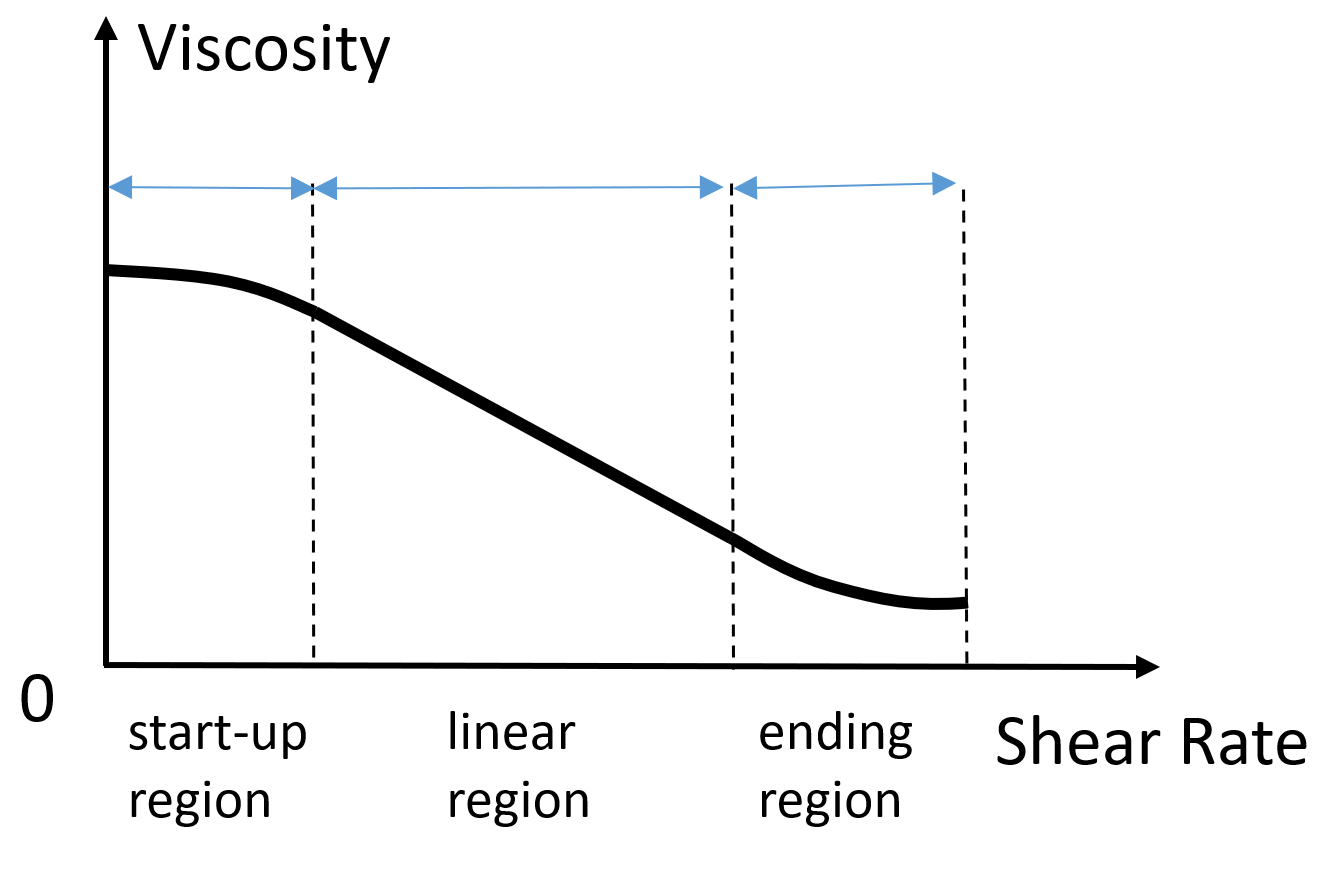
\includegraphics[width=0.6\textwidth]{pics/reverse-S.png}
	\captionsetup{labelformat=empty}
	\caption{Figure 6: The reverse-S shape viscosity-shear-rate curve for Cross Model and Carreau Model.}
\end{figure}



% ----------------------------- reviewer 1 comment 14 ---------------------------- %

\vspace{0.4cm}
\noindent$\bullet$ \enspace \textbf{Comment 14:}
\textit{Hooke's name should have an 'e' at the end.}

\vspace{0.2cm}
\textbf{Response:}
Thank you. We have corrected this error.

% ----------------------------- reviewer 1 comment 15---------------------------- %

\vspace{0.4cm}
\noindent$\bullet$ \enspace \textbf{Comment 15:}
\textit{Stylistically, I would recommend not adopting these odd abbreviations (shao22, fang19, su21). Or, at least capitalize them consistently with how they are later used. }

\vspace{0.2cm}
\textbf{Response:}
Thank you for your kind suggestion. We apologize for any confusion caused. In the revised manuscript, we will replace the ambiguous references with the specific names of the frameworks, i.e., FLIP and MPM. And we will ensure that the caption and corresponding text clearly indicate which MPM model we are referring to (Su's or Fang's). The related experiments in the video will also be updated accordingly.


% ----------------------------- reviewer 1 comment 16 ---------------------------- %

\vspace{0.4cm}
\noindent$\bullet$ \enspace \textbf{Comment 16:}
\textit{There is a spurious indent after Eq. 31.}

\vspace{0.2cm}
\textbf{Response:}
Thank you for your careful review. We have corrected this mistake.

% ----------------------------- reviewer 1 comment 17 ---------------------------- %

\vspace{0.4cm}
\noindent$\bullet$ \enspace \textbf{Comment 17:}
\textit{How is cutting actually performed? Presumably the particles need to be at least some minimum distance apart for them not to interact? Does cutting push them apart? Or does the cutting tool block them from communicating? Otherwise removing the cutting tool would allow them to reconnect and then fail to separate. }

\vspace{0.2cm}
\textbf{Response:}
Thank you for the comments. Actually, we insert the cut board into the chocolate bunny. This cut board is also composed of particles and has a certain thickness. So your guess is correct. The inserted cut board causes the particles in the chocolate bunny to separate, which makes the particles travel further than the neighbourhood search threshold, producing the separating effect. To give readers a better understanding, we added the following explanation to our revised manuscript:

\vspace{0.2cm}
\textbf{Revised text:}

\revised{
The cutting phenomenon is realized by the insertion of the cutting board, which is composed of particles and has a certain thickness. The board divides the bunny particles to disperse, leading them to travel beyond the neighbourhood search threshold, thereby creating the separating effect.}


% ----------------------------- reviewer 1 comment 18 ---------------------------%

\vspace{0.4cm}
\noindent$\bullet$ \enspace \textbf{Comment 18:}
\textit{ The motion of the liquid surface at the time of impact in the golf ball test looks a bit odd to me. Perhaps it is the rendering, but I cannot quite tell what is happening around that time. A slow motion visualization might be helpful to clarify?  }

\vspace{0.2cm}
\textbf{Response:}
Thank you for the comments. We apologize for the confusion caused. At the moment of collision, there is a sudden increase in shear rate, which causes an immediate surge in viscosity within the collision region. Consequently, the ball does not drop right away. However, this process is relatively short-lived. Following this, the ball gradually begins to sink. This is due to the fact that the shear rate reverts to a lower level, causing the viscosity to also return to a lower level. Thus, under the influence of gravity, the ball starts to sink slowly, beginning at a lower velocity. As you suggested, we have slowed down the collision moment (0.2X speed) in the video and re-rendered the variation of shear rate to provide better clarity.

% ----------------------------- reviewer 1 comment 19 ---------------------------- %

\vspace{0.4cm}
\noindent$\bullet$ \enspace \textbf{Comment 19:}
\textit{I could not understand quite what the comment about tree trunk particles and meadow particles was talking about (p8, right column). The last paragraph before section 6 seems to emphasize AR/VR. Is this just a hold-over from the earlier submission to an AR/VR conference? Should this be removed/modified? Also same later in Section 6.  }

\vspace{0.2cm}
\textbf{Response:}
We apologize for the confusion. As per your comments, we realize that the VR painting experiment has less business with our non-Newtonian framework. Per your suggestion above, the VR-related content and experiments have been deleted in our revised version.

% ----------------------------- reviewer 1 comment 20 ---------------------------- %

\vspace{0.4cm}
\noindent$\bullet$ \enspace \textbf{Comment 20:}
\textit{In Figure 12, Newtonian is capitalized strangely (NewTonian) }

\vspace{0.2cm}
\textbf{Response:}
Thank you for your careful review. We have corrected this error.

% ----------------------------- reviewer 1 comment 21 ---------------------------- %

\vspace{0.4cm}
\noindent$\bullet$ \enspace \textbf{Comment 21}
\textit{Suggesting references}

\textit{"An implicit compressible SPH solver for snow simulation"
}

\textit{"Melting and Flowing"}


\vspace{0.2cm}
\textbf{Response:}
Thank you for your suggestion. We have added these two references relevant closely to our work.

\vspace{0.2cm}
\textbf{Added text:}

\revised{Gissler et al.~\cite{Gissler2020-snow} simulated the snow with SPH. Their work refers to the visco-elastic model built by Stomakin et al.~\cite{Stomakhin2014}.}

\revised{Carlson et al.~\cite{Carlson2002} enhanced the numerical stability of algorithms under high viscosity for simulating phenomena such as wax melting.}



We sincerely appreciate your careful reviews and suggestions which help us greatly improve the manuscript. We hope you are satisfied with our revision, and we can get your final acception.



% ---------------------------------------------------------------------------- %
%                                   reviewer2                                  %
% ---------------------------------------------------------------------------- %
\newpage
\vspace{-1.5cm}
\begin{flushleft}
	\textit{\textbf{Responses to the Comments from Reviewer 2}}
\end{flushleft}


% ----------------------------- reviewer 2 comment 1 ---------------------------- %

\vspace{0.4cm}
\noindent$\bullet$ \enspace \textbf{Comment 1:}
\textit{I first thought it was nice that the authors introduce the Generalized Maxwell Model (GMM) shown in Fig. 2, which is (to the best of my knowledge) not very popular in the graphics community yet. However, I could not find a suitable reference to the GMM model in the manuscript. I just noticed the GMM model is rather popular for viscoelasticity without plasticity. I am not sure if the presented one is the well-known GMM or an adapted model for plasticity. The presented model looks similar to the visco-elasto-plasticity model proposed by [Fang et al. 2019]. The author should clarify this.}


\vspace{0.2cm}
\textbf{Response:}
Thank you very much for your valuable comments.
Our GMM model is an 'adapted model for plasticity' that has been modified by ourselves. As you rightly pointed out, GMM is primarily used for viscoelastic materials. We drew inspiration from the ideas presented by Fang et al.~\cite{Fang2019-sillyRubber}. In addition, we have expanded their GMM model by incorporating plasticity, enabling us to handle a variety of non-Newtonian behaviors.

As per what you suggested, we have added the following text to point out the origin of the GMM concept.

\vspace{0.2cm}
\textbf{Added text:}

\revised{We present a Generalized Maxwell Model to describe the constitutive relation underlying our unified non-Newtonian framework. Our inspiration is from the similar model from Fang et al.[32] for viscoelasticity simulation.}



% ----------------------------- reviewer 2 comment 2 ---------------------------- %

\vspace{0.4cm}
\noindent$\bullet$ \enspace \textbf{Comment 2:}
\textit{The performance comparisons with FLIP and MPM need further clarification. Both FLIP and MPM are hybrid methods, which use both grid and particles. The grid information, which is an important factor for their performance, is missing; thus, I was not fully convinced of the performance superiority of the proposed method. }


\vspace{0.2cm}
\textbf{Response:}
Thank you for your comments. We agree with your viewpoint. With regard to performance comparisons, our non-Newtonian framework indeed does not showcase superior performance. As we acknowledged in the Limitations Section, we did not specifically optimize for performance. To make a more fair comparison, we recognize the need to reconfigure the performance experiments. Consequently, in the updated manuscript, we introduced a new comparison for the Honey and Toy Cow scenes. We kept the particle count roughly the same and came to the same conclusion: for visco-elastic-plastic behavior simulation, our method is roughly equivalent to FLIP and superior to MPM; for viscous behavior simulation, our method has the best efficiency. Overall, our method has the relatively highest cost performance as it could cover more phenomena while maintaining acceptable efficiency.
Thanks so much for your kind suggestion to make experiments more rigorous and convincing. We have made adjustments to the relevant discussion.

The new performance table is as follows:
\begin{table}[H]
	\centering
        \captionsetup{labelformat=empty}
	\caption{\revised{Table: Performance comparison with existing works.}} \label{tab:performance1}
	\definecolor{cyan}{rgb}{0,0,0}
	\begin{tblr}{
		width = \linewidth,
		colspec = {Q[250]Q[146]Q[204]Q[158]Q[158]},
		row{2} = {c},
		cell{1}{1} = {r=2}{},
		cell{1}{2} = {c},
		cell{1}{3} = {c},
		cell{1}{2} = {c=2}{0.35\linewidth},
		cell{1}{4} = {c=2}{0.316\linewidth},
		cell{3}{2} = {c},
		cell{3}{3} = {c},
		cell{3}{4} = {c},
		cell{3}{5} = {c},
		cell{4}{2} = {c},
		cell{4}{3} = {c},
		cell{4}{4} = {c},
		cell{4}{5} = {c},
		cell{5}{2} = {c},
		cell{5}{3} = {c},
		cell{5}{4} = {c},
		cell{5}{5} = {c},
		hline{1} = {-}{},
		hline{2} = {2-5}{cyan},
		hline{3,6} = {-}{cyan},
			}
		\textbf{Method}                                & \textbf{Time(s)/frame} &                                & \textbf{Particles number} &                                  \\
		                                               & \textbf{Cow}           & \textbf{Honey}                 & \textbf{Cow}              & \textbf{Honey}                   \\

		\textbf{FLIP}~\cite{Shao-Huang2022-unsmoothed} & \bf \underline{0.44}  & {0.06}               & {275,556}                   & \revised{13,815}                 \\
		\textbf{MPM}~\cite{Fang2019-sillyRubber}       & 23.4                   & {11.6}               & 274,462                   & \revised{13,860}                 \\
		\textbf{SPH (ours)}                            & 22.7                   & \bf \underline{\revised{0.04}} &  {276,625}   &  {\revised{13,780}}
	\end{tblr}
\end{table}


% ----------------------------- reviewer 2 comment 3 ---------------------------- %

\vspace{0.4cm}
\noindent$\bullet$ \enspace \textbf{Comment 3:}
\textit{In the Honey (Fig. 7) example, the authors claim that the compared MPM does not achieve the desired high-viscous behavior despite being known to support high-viscous materials. It would be better to elaborate more on why this was the case in the presented test. I am wondering if it is a boundary handling issue, material parameter issue, simulation resolution issue, or something else. }


\vspace{0.2cm}
\textbf{Response:}
Thank you for your helpful comments. We apologize for the inaccuracy of this comparison experiment. We have re-simulated the scene, and this time we obtained consistent viscous effect among these three methods (as shown in the following figure and Fig. 8 in our revised paper). Furthermore, we have constrained the number of particles to a uniform level (all at 13.8K). After the re-simulation, we found that FLIP takes 0.06s per frame, our SPH takes 0.04s, while MPM takes 11.6s. Therefore, the conclusion remains unchanged: our framework performs on par with FLIP and both outperform MPM.


\begin{figure}[htbp]
	\centering
	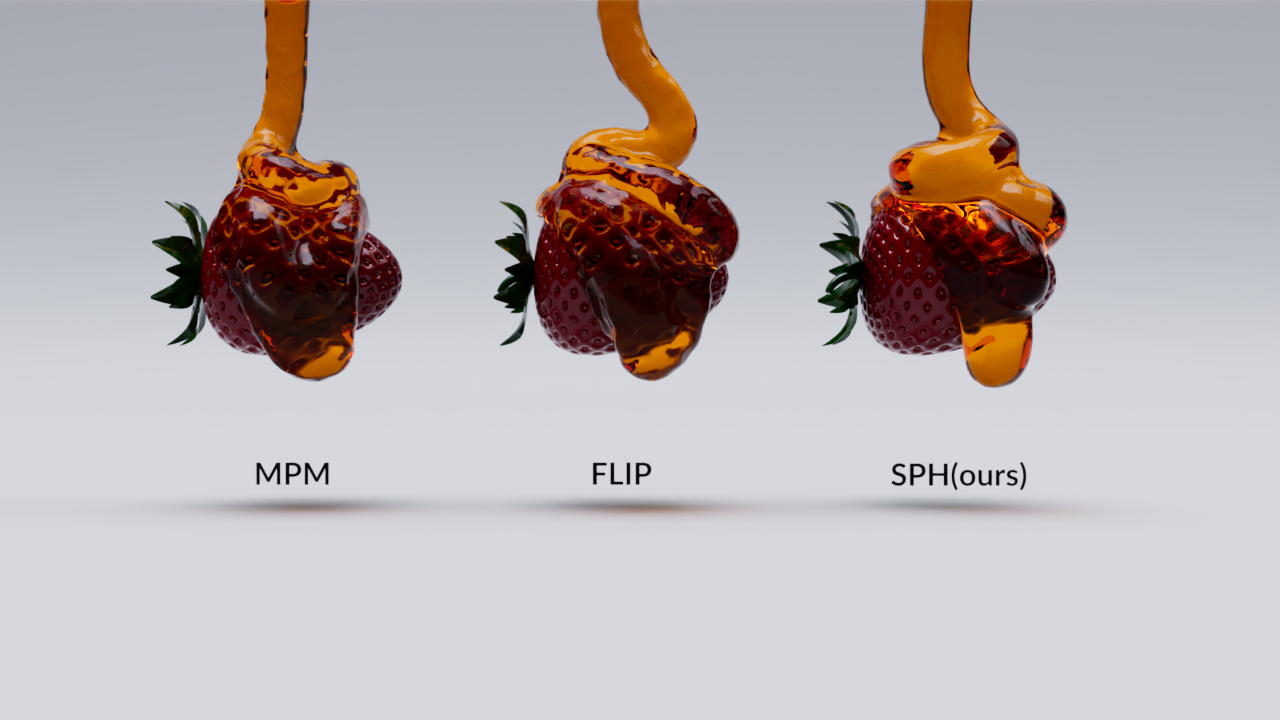
\includegraphics[width=0.6\textwidth]{pics/honey_comp.png}
	\captionsetup{labelformat=empty}
	\caption{\revised{Figure 8: Comparisons of highly viscous behaviors. From left to right, there are three phenomena of honey dripping modeled by MPM (Fang et al.), FLIP (Shao et al.) and our framework, respectively.}}
\end{figure}


% ----------------------------- reviewer 2 comment 4 ---------------------------- %

\vspace{0.4cm}
\noindent$\bullet$ \enspace \textbf{Comment 4:~\label{Armadillos}}
\textit{In the Armadillos (Fig. 12) example, it is nice to see such a large variety of different models. On the other hand, however, it is less intuitive regarding what kinds of materials/behaviors are intended. It would be better to elaborate to give a more intuitive explanation of such different models.  }

\vspace{0.2cm}
\textbf{Response:}
Thank you for your suggestion. We have added the following text to give an intuitive explanation for armadillos example as you suggested.

\vspace{0.2cm}
\textbf{Added text:}

\revised{In this experiment, we evaluate seven distinct viscosity models that are related to shear rate. The viscosity models depicted in Fig.~14 include Carreau, Casson, Cross, PowerLaw2 (shear-thickening), PowerLaw1 (shear-thinning), Newtonian, Herschel-Bulkley, and Bingham models. These models can be classified into four categories: 1) Shear-thinning behaviors, which include Carreau, Cross, and PowerLaw1; 2) Shear-thickening behavior, primarily represented by PowerLaw2; 3) Bingham behavior, including Herschel-Bulkley, Bingham, and Casson; and 4) Newtonian behavior~\cite{Chhabra2010,Phan2017}}.

%\revised{It's important to note that the PowerLaw model can be subdivided into PowerLaw1 (shear-thinning) and PowerLaw2 (shear-thickening). This is because adjusting the parameter $n$ can emulate various non-Newtonian behaviors, such as shear-thinning ($n<1$) and shear-thickening ($n>1$). }

\revised{As shown in Fig.~14, it's clear that PowerLaw2 (shear-thickening) exhibits the optimal flowability. This is due to the fact that it simulates shear-thickening behavior, where viscosity escalates with the increase of shear rate. In our experiment, the high-viscosity fluid begins flowing from zero velocity under the influence of gravity, at a relatively low shear rate. At low shear rates, the viscosity remains low. }

\revised{In contrast, PowerLaw1 (shear-thinning) exhibits the least flowability. This is due to its simulation of shear-thinning behavior under the same parameters as PowerLaw2 (with the exception of $n$). Consequently, at low shear rate, the viscosity remains high.}

%\revised{The Bingham model demonstrates moderate flowability, similar to the Newtonian model. The defining feature of the Bingham model is that the fluid exhibits rigidity until the yield point is surpassed. Beyond that, its behavior aligns with that of a typical Newtonian fluid. For the Bingham model, the stress-strain curve beyond the yield point mirrors that of the Newtonian model.}
%\revised{It is important to note that the concept of Bingham behavior mentioned in this study is distinct from the Bingham model. The former refers to stress-strain curves with a yield point, while the latter specifically refers to the simplest model that simulates Bingham behavior, which exhibits Newtonian behavior once it exceeds the yield point.}
\revised{There are two models used for simulating Bingham behavior: the Herschel-Bulkley model and the Casson model. Beyond the yield point, the Herschel-Bulkley model adheres to PowerLaw behavior, which could manifest as shear-thinning, shear-thickening, or Newtonian. Consequently, it offers more flexibility and has a greater number of parameters. As demonstrated in Fig.~14, this model exhibits behavior similar to that of a Newtonian fluid. Conversely, the Casson model is only capable of simulating shear-thinning Bingham behavior. Therefore, in agreement with our analysis of PowerLaw1 (shear-thinning), the fluid flowability simulated by the Casson model is relatively poor at low shear rate.}

\revised{The Carreau model and the Cross model~\cite{Cross1965} are used to simulate shear-thinning behaviors. These two models are somewhat similar, with their stress-strain curves displaying a reverse S-shaped pattern. Specifically, at both low and high shear rates, the constitutive curves tend to level out. Therefore, even though both models are used to simulate shear-thinning behavior similar to PowerLaw1, the viscosity at low shear rates doesn't reach the high levels observed with PowerLaw1, resulting in moderate flowability.}


\begin{figure}[htbp]
	\centering
	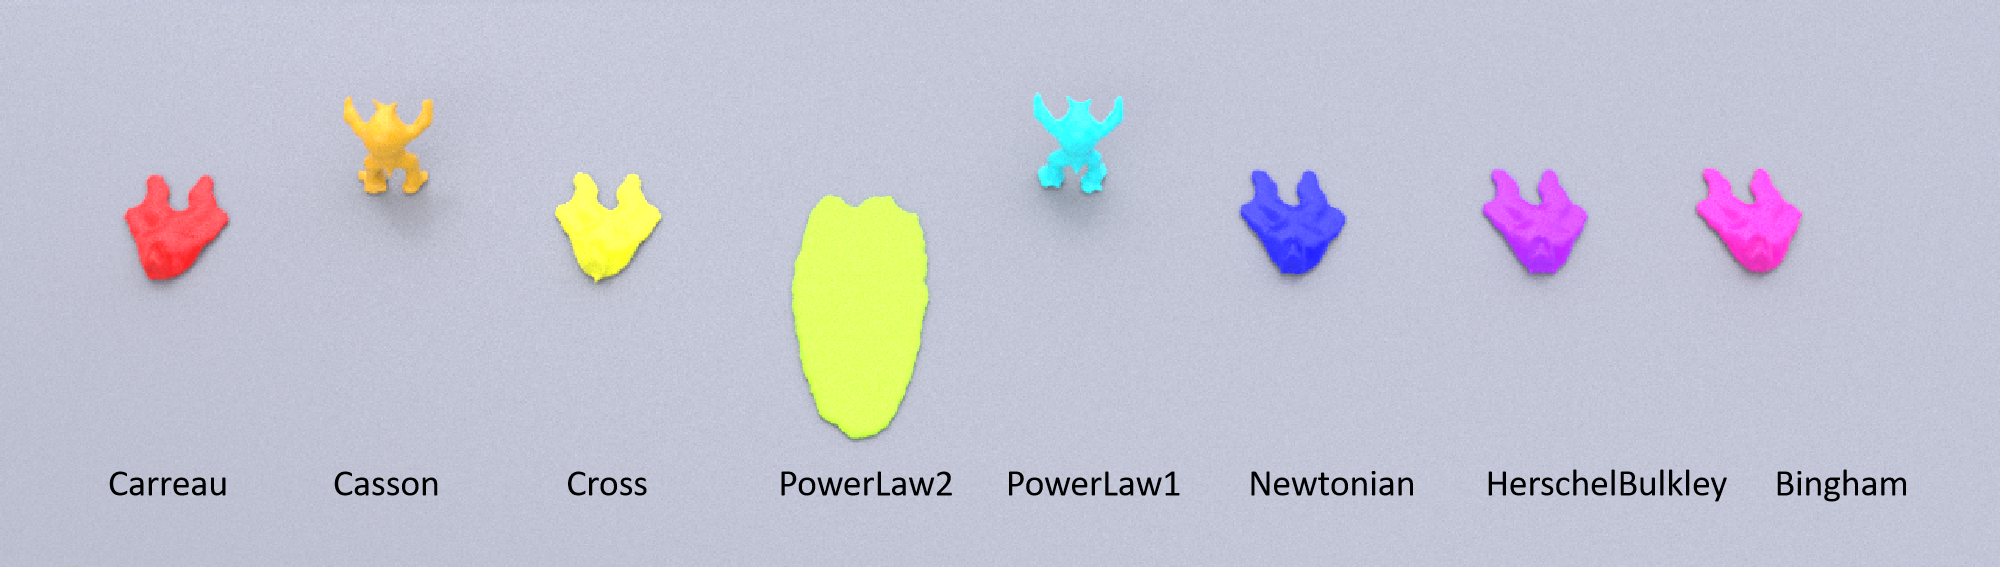
\includegraphics[width=0.85\textwidth]{pics/ramp.png}
	\captionsetup{labelformat=empty}
	\caption{\revised{Figure 14. Armadillos with different strain-rate-dependent non-Newtonian viscosity model. From left to right: Carreau, Casson, Cross, PowerLaw2, PowerLaw1, Newtonian, Herschel-Bulkley, Bingham. Detailed parameters are listed in Table 4.}}
\end{figure}



% ----------------------------- reviewer 2 comment 5 ---------------------------- %

\vspace{0.4cm}
\noindent$\bullet$ \enspace \textbf{Comment 5:}
\textit{For example, I was pleased to see the example of shear-thickening in Fig. 11 for a cornstarch mixture, yet, at the same time, I was wondering about the other materials, for instance, ketchup, simulated in this setup. }


\vspace{0.2cm}
\textbf{Response:}
Thank you for your comments. Following your suggestion, we have included an experiment with the same setup as the cornstarch mixture case (Fig. 12 in our manuscript), but with the fluid changed to ketchup (Fig. 13 in our manuscript). 


\vspace{0.2cm}
\textbf{Added text:}

\revised{ To compare the shear-thinning and shear-thickening behaviors, we substitute the fluid with ketchup (a shear-thinning fluid) and a golf ball falls into ketchup, while retaining other setup parameters. We adapt its parameters from~\cite{Bottiglieri1991}, using a power law model (n=0.26, m=5.86, parameters can be found in Table~3). Due to its shear-thinning nature, the viscosity decreases at the moment of collision, resulting in a splashing effect.}

\begin{figure*}[htbp]
	\centering
	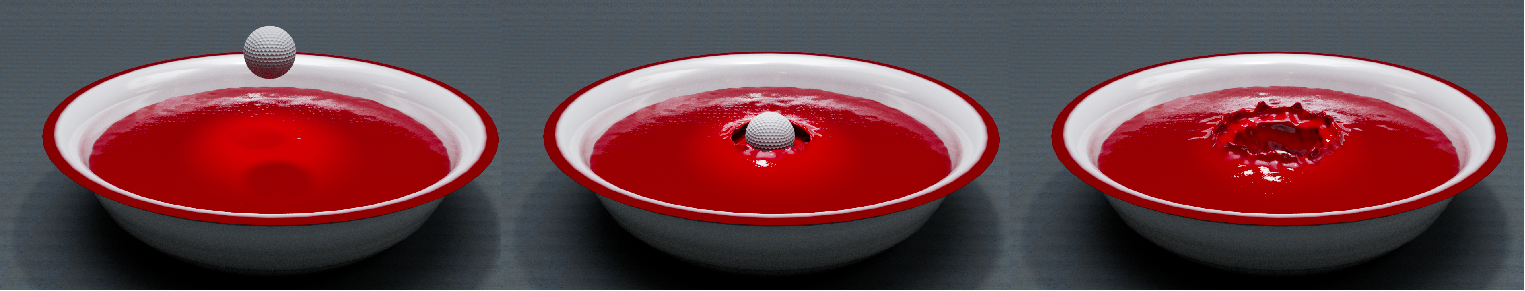
\includegraphics[width=0.95\textwidth]{pics/ketchup.png}
	\captionsetup{labelformat=empty}
	\caption{\revised{Figure 13. Change the fluid to ketchup (which is shear-thinning) and keep other setups the same with golf smashing cornstarch-water mixture case (Fig. 12).}} 
\end{figure*}


% ----------------------------- reviewer 2 comment 6 ---------------------------- %

\vspace{0.4cm}
\noindent$\bullet$ \enspace \textbf{Comment 6:}
\textit{Additionally, I don't think it's necessary to show the first row of Fig. 12. }


\vspace{0.2cm}
\textbf{Response:}
Thank you for your kind suggestion, we have deleted the first row of Fig.12.

% ----------------------------- reviewer 2 comment 7 ---------------------------- %

\vspace{0.4cm}
\noindent$\bullet$ \enspace \textbf{Comment 7:}
\textit{In the video for shear-thickening (Fig. 11), I found that the particle colors, indicating the strain rate, changed before the ball hit the fluid surface. Why does it happen before the actual interaction? }


\vspace{0.2cm}
\textbf{Response:}
We apologize for any confusion caused. The discrepancy arises due to post-processing during rendering. In the simulation process, it isn't feasible or necessary to include golf balls with textured and uneven surfaces. Instead, we use a discretized sphere composed of particles for the actual simulation. During the rendering process, we replace the simulated sphere with a textured golf ball that has uneven surfaces. We feel sorry that there may be differences between the rendered ball's position and the actual simulation results.
Thanks to your careful review, we have implemented adjustments to our rendering in the updated video.


% ----------------------------- reviewer 2 comment 8 ---------------------------- %

\vspace{0.4cm}
\noindent$\bullet$ \enspace \textbf{Comment 8:}
\textit{The exposition could be further improved by revising the following:
	\begin{enumerate}
		\item  In Section 4.3, there are some repeated phrases regarding the Lagrangian framework.
		\item  In Fig 5, the first two lines are not easy to distinguish in color.
		\item  On page 4, line 59, the right column: there is a typo "... approaches ..."
		\item On page 8, line 53, the right column: "physics  meaningful" sounds unnatural.
		\item On page 9, line 42, the right column: "overallly" sounds unnatural.
		\item Bold faces of math symbols for matrices and vectors are not consistent.
		\item Referring to equations in the text is not consistent, e.g., "Eq. 3" or "Eq.(22)".
	\end{enumerate}
}


\vspace{0.2cm}
\textbf{Response:}
Thank you very much for your careful review and helpful suggestions. We have corrected all the above errors and checked throughout the entire manuscript to eliminate typos and improper descriptions to the best of ability. 





% ----------------------------- reviewer 2 comment 9 ---------------------------- %

\vspace{0.4cm}
\noindent$\bullet$ \enspace \textbf{Comment 9:}
\textit{For the supplemental video: Some examples used colormaps. It would be better to indicate what the colors mean when it's presented.}


\vspace{0.2cm}
\textbf{Response:}
We are sorry for the confusion. We have added a color map in the revised video and explained its meaning in detail to avoid any confusion.



% ----------------------------- reviewer 2 comment 10 ---------------------------- %

\vspace{0.4cm}
\noindent$\bullet$ \enspace \textbf{Comment 10:}
\textit{Suggesting references:}
\begin{itemize}

	\item \textit{Bargteil et al., A finite element method for animating large viscoplastic flow, SIGGRAPH 2007,}

	\item \textit{Wojtan and Turk, Fast viscoelastic behavior with thin features, SIGGRAPH 2008,}

	\item \textit{Andrade et al., Particle-based fluids for viscous jet buckling, C\&G 2015,}

	\item \textit{Yue et al., Continuum foam: A material point method for shear-dependent flows, TOG 2015,}

\end{itemize}



\vspace{0.2cm}
\textbf{Response:}
Thank you for your suggestion. We have added these references in our revised manuscript.


\vspace{0.2cm}
\textbf{Added text:}

\revised{Bargteil et al.~\cite{Bargteil-2007-AFE} used FEM to simulate the visco-plastic flow. To tackle the potential problem of the ill-conditioned ill-conditioned mesh after large deformation, they used a re-mesh procedure.}

...

\revised{Wojtan and Turk~\cite{Wojtan2008} took a similar strategy with Barteil et al. to simulate the visco-elastic behavior. They carefully distinguished the situation for remeshing. With the spatial adaptivity technique, their algorithm achieves an order-of-magnitude speedup.}

...

\revised{Andrade et al.~\cite{Andrade2015} utilized a SPH based method to simulate the non-Newtonian viscosity with Cross model and accelerated the performance with CUDA.}

...

\revised{Yue et al.~\cite{Yue2015} used MPM to simulate the foam, which is a typical Bingham type non-Newtonian material. Their constitutive correlation is based on the Herschel-Bulkley model. }


Thank you very much for your positive reviews, and we hope you are satisfied with our
revisions.



% ---------------------------------------------------------------------------- %
%                                   reviewer3                                  %
% ---------------------------------------------------------------------------- %
\newpage
\vspace{-1.5cm}
\begin{flushleft}
	\textit{\textbf{Responses to the Comments from Reviewer 3}}
\end{flushleft}


% ----------------------------- reviewer 3 comment 1 ---------------------------- %
\vspace{0.4cm}
\noindent$\bullet$ \enspace \textbf{Comment 1:}
\textit{First, I do not really understand the emphasis on the fact, that the concept is a "unified" particle approach. I basically see one material and particles are used in the discretization. I do not see that there would be the option of a non-unified particle approach for this one material in contrast to the advertised unified approach. }


\vspace{0.2cm}
\textbf{Response:}
Thank your very much for your careful review and helpful comments. We feel quite sorry about confusion caused by the use of the word "unified". In simple terms, "unified" means that we are combining all non-Newtonian behaviors (viscous, elastic, and plastic) in a framework.

In our literature review, we found that there are few existing methods specifically designed for studying non-Newtonian behaviors. Technically speaking, any behavior that doesn't adhere to the Newtonian shear law is classified as non-Newtonian. However, this definition is expansive and nebulous. Resorting to the rheological definition falls short of the requirements for visual effects in computer graphics. According to our analysis, the key to showcasing the visual effect of non-Newtonian behaviors lies in demonstrating the material’s dynamic characteristics ranging from fluid-like to solid-like. Therefore, a simulation algorithm needs to consider the following key features: 1) variable viscosity (encompassing classical shear-related models), 2) the incorporation of elasticity, and 3) the inclusion of plasticity.

%Existing research rarely covers all of the above points. Early works such as Carlson~\cite{Carlson2002} and Stora~\cite{Stora1999} considered classical shear-related variable viscosity models. Zhu~\cite{Zhu2015-nonNewton} is one of the few papers dedicated to simulating non-Newtonian behaviors, considering variable viscosity and elasticity. However, it only provides one shear-related variable viscosity model and lacks plasticity simulation. In recent years, some works using Material Point Method (MPM) claim to be capable of simulating non-Newtonian behaviors, such as Su~\cite{Su2021} and Fang~\cite{Fang2019-sillyRubber}. However, their methods are only focused on viscoelastic behavior. Solenthaler~\cite{Solenthaler2009-PCISPH} proposed a unified SPH-based approach that could simulate both fluids and solids, but it did not specifically address viscoelastic materials in-between fluids and solids. Goktekin~\cite{Goktekin2004} simulated semi-fluid, semi-solid materials by adding elastic stress in the momentum equation, which provided us some inspiration. Our elastic approach is inspired by Becker~\cite{Becker2009}, and the plasticity approach is inspired by O'Brien~\cite{OBrien2002}. However, these are individual works. 
In the field of computer graphics, we have not seen specialized research that covers the majority of non-Newtonian behaviors, despite the fact that non-Newtonian behaviors are widely present in real-world phenomena. Therefore, we believe that there is a need for an approach that unifies the three aforementioned behavioral characteristics.
Thanks to your valuable comment, to avoid the potential confusion of readers, we have supplemented the explanation in our revised manuscript as follows:

\vspace{0.4cm}
\textbf{Added Text:}

\revised{For computer graphics applications, the key to depicting the visual effect of non-Newtonian behaviors is to demonstrate the material’s dynamic characteristics, which can range from fluid-like to solid-like. Hence, a simulation algorithm needs to consider the following key features: 1) variable viscosity (incorporating classical shear-related models), 2) the inclusion of elasticity, and 3) the integration of plasticity.}

\revised{
Existing research seldom covers all of the above-mentioned research issues. Early works, such as Carlson et al.~\cite{Carlson2002} and Stora et al.~\cite{Stora1999}, considered classical shear-related variable viscosity models. The work of Zhu et al.~\cite{Zhu2015-nonNewton} is among the few papers dedicated to simulating non-Newtonian behaviors, taking into account variable viscosity and elasticity. However, it only offers one shear-related variable viscosity model and lacks plasticity simulation. In recent years, some works using the Material Point Method (MPM), such as Su et al.~\cite{Su2021} and Fang et al.~\cite{Fang2019-sillyRubber}, claim to be able to simulate non-Newtonian behaviors. However, their methods primarily focus on viscoelastic behavior. Solenthaler et al.~\cite{Solenthaler2007} proposed a unified SPH-based approach that could simulate both fluids and solids, but it did not specifically address viscoelastic materials that lie between fluids and solids. Goktekin et al.~\cite{Goktekin2004} simulated semi-fluid, semi-solid materials by adding elastic stress in the momentum equation, which offered us some inspiration. 
 However, we haven't seen specialized research that encompasses the majority of non-Newtonian behaviors, despite the fact that non-Newtonian behaviors are widely observed in real-world phenomena. As such, we believe that consolidating the three aforementioned behavioral characteristics (viscous, elastic, and plastic) into a unified framework will represent a significant contribution to the computer graphics community, at least at the application level. }
 
% ----------------------------- reviewer 3 comment 2 ---------------------------- %
\vspace{0.4cm}
\noindent$\bullet$ \enspace \textbf{Comment 2:}
\textit{My second point would be about the experiments. The paper presents numerous experiments and analyses, which is definitely sufficient for a publication. On the other hand, I am wondering, wether a short discussion of extreme cases for the parameterization of the material model might be interesting. This could also be seen as a discussion of limitations.  }


\vspace{0.2cm}
\textbf{Response:}
Thank you for your comments. We wholeheartedly agree with your perspective, as in-depth discussion and analysis will undoubtedly enhance the quality of our article. In numerous instances, extreme parameter choices may culminate in non-convergent results. For example, excessively quick changes in viscosity and overly large values of the elastic modulus might lead to such outcomes. Some scenarios result in numerical explosions right from the outset, while others encounter such issues midway. The numerical explosions are likely due to abrupt variations in certain parameters. For instance, the moment the golf ball collides with the fluid in the falling golf ball scenario can trigger a sudden change in viscosity, resulting in a breakdown. Similarly, in the case of a falling elastic tomato, if the elastic modulus is set too high, the program will crash immediately. We speculate that these extreme situations may be linked to numerical stiffness issues. Therefore, a stable viscosity and elastoplastic solver may be the key to resolving these problems. We anticipate further and much more in-depth explorations of the aforementioned topics will occur in the near future. 

As per your suggestion, we have added the following paragraph in the Section Limitation:

\vspace{0.2cm}
\textbf{Added text:}

\revised{We also observed that unreasonable extreme parameters may lead to the non-convergence of numerical simulations. For example, rapidly changing viscosity and excessively large elastic modulus can cause issues such as numerical explosion. 
%Some examples result in numerical explosions from the beginning, while others may experience a numerical explosion in the middle. The occurrence of a explosion in the middle is likely due to sharp variations in certain parameters. 
For instance, the moment the golf ball collides with the fluid in the falling golf ball scenario will trigger a sudden change in viscosity, which may result in a breakdown. Similarly, in the case of a falling elastic tomato, if the elastic modulus is set extremely high, the program will crash immediately. We speculate that these extreme situations may be attributed to numerical stiffness issues. Therefore, a stable viscosity and elastoplastic solver may be the key to resolving these problems. We anticipate further exploration in this area in future work.}

% ----------------------------- reviewer 3 comment 3 ---------------------------- %

\vspace{0.4cm}
\noindent$\bullet$ \enspace \textbf{Comment 3:}
\textit{Suggesting references:}
\begin{itemize}
	\item \textit{Peer's Prescribed Velocity Gradients for Highly Viscous SPH Fluids with Vorticity Diffusion (IEEE TVCG 2017) }
\end{itemize}


\vspace{0.2cm}
\textbf{Response:}
Thank you for your suggestion. We have added this relevant reference in our revised manuscript. 


\vspace{0.2cm}
\textbf{Added text:}

\revised{Similarly, Peer and Teschner et al.~\cite{Peer2017-Prescribed} used the prescribed velocity gradient to simulate the viscous fluid.}


We sincerely appreciate your thorough reviews and valuable suggestions which have immensely helped us enhance the manuscript. We hope that our revisions meet your expectations and we look forward to receiving your final acceptance.

% ---------------------------------------------------------------------------- %
%                                   reviewer4                                  %
% ---------------------------------------------------------------------------- %
\newpage
\vspace{-1.5cm}
\begin{flushleft}
	\textit{\textbf{Responses to the Comments from Reviewer 4}}
\end{flushleft}



% ----------------------------- reviewer 4 comment 1 ---------------------------- %
\vspace{0.4cm}
\noindent$\bullet$ \enspace \textbf{Comment 1:}
\textit{Regarding the shear-thickening behavior, one reference is mentioned as above, the author should also discuss it in the revised version.}

\textit{An SPH model to simulate the dynamic behavior of shear thickening fluids. Oktar Ozgen et al, 2019.}

\vspace{0.2cm}
\textbf{Response:}
Thank you immensely for your careful review and constructive feedback. In accordance with your suggestion, we acknowledged that the recommended paper is pertinent to our work. Consequently, we have included the reference in the 'Related Works' Section.

\vspace{0.2cm}
\textbf{Added text:}

\revised{Ozgen et al.~\cite{Ozgen2019} simulated the behavior of shear thickening fluids with SPH model. The key factor in their method is to use a spring to reproduce the nonlinearity of the non-Newtonian behavior.}


% ----------------------------- reviewer 4 comment 2 ---------------------------- %
\vspace{0.4cm}
\noindent$\bullet$ \enspace \textbf{Comment 2:}
\textit{The main contribution of this paper is incremental and inspiring. The implementation of unified solver collects previous known models and incorporated it. I am glad to see different non-Newtonian simulation can be done in one framework. However, as I mentioned above, the necessity of a unified solve is not clearly demonstrated. The author should discuss this in the revised version.}



\vspace{0.2cm}
\textbf{Response:}
Thank you for comments. As per you suggested, we realized that explaining and emphasizing the necessity of “a unified solve” is very important.

Some of the existing researches focus on the individual performance of non-Newtonian behaviors, such as Carlson et al.~\cite{Carlson2002} and Stora et al.~\cite{Stora1999}, considered classical shear-related variable viscosity models. Zhu et al.~\cite{Zhu2015-nonNewton} took into account variable viscosity and elasticity, it offers only one shear-related variable viscosity model and does not include plasticity simulation. Su et al.~\cite{Su2021} and Fang et al.~\cite{Fang2019-sillyRubber} simulated non-Newtonian behaviors with the popular MPM model. However, their methods primarily concentrate on viscoelastic behavior. Solenthaler et al.~\cite{Solenthaler2009-PCISPH} proposed a unified SPH-based approach capable of simulating both fluids and solids, but it did not specifically address viscoelastic materials that fall between fluids and solids. Goktekin~\cite{Goktekin2004} simulated semi-fluid, semi-solid materials by incorporating elastic stress into the momentum equation. 

Despite the wide prevalence of non-Newtonian behaviors in real-world phenomena, we have yet to see specialized computer graphics research that could encompass the various non-Newtonian behaviors in a unified solver. The challenges remain that non-Newtonian key features (variable viscosity, incorporation of elasticity, inclusion of plasticity) can hardly coordinate and synchronize in a seamless manner.   
 Therefore, we believe that a flexible but unified framework, which allows for the coupling of these features, would be a significant and useful addition to the computer graphics research.

Per your valuable comments above, we have added the explanation in our revised manuscript:

\vspace{0.4cm}
\textbf{Added Text:}

\revised{For computer graphics applications, the key to depicting the visual effect of non-Newtonian behaviors is to demonstrate the material’s dynamic characteristics, which can range from fluid-like to solid-like. Hence, a simulation algorithm needs to consider the following key features: 1) variable viscosity (incorporating classical shear-related models), 2) the inclusion of elasticity, and 3) the integration of plasticity.}

\revised{
 ... \\
However, we haven't seen specialized computer graphics research that encompasses the majority of non-Newtonian behaviors, despite the fact that non-Newtonian behaviors are widely observed in real-world phenomena. As such, we believe that consolidating the three aforementioned behavioral characteristics (viscous, elastic, and plastic) into a unified framework will represent a significant contribution to the computer graphics community.}

% ----------------------------- reviewer 4 comment 3 ---------------------------- %
\vspace{0.4cm}
\noindent$\bullet$ \enspace \textbf{Comment 3:}
\textit{In section 5.3, the dynamic behavior of different viscous models could be more discussed.}


\vspace{0.2cm}
\textbf{Response:}
Thank you for your suggestion. As you and Reviewer 2 suggested, we have added more discussion. Please refer to our Response in \hyperref[Armadillos]{Comment 4 of Reviewer 2}. In the interest of space, no need to repeat here. Thank you. 

% ----------------------------- reviewer 4 comment 4 ---------------------------- %
\vspace{0.4cm}
\noindent$\bullet$ \enspace \textbf{Comment 4:}
\textit{In section 5.4, the elastic case of the failing tomato shows unnatural trembling, please discuss this.}


\vspace{0.2cm}
\textbf{Response:}
Thank you for pointing out the problem. Indeed, this trembling does exist. We observed this trembling phenomenon in cases involving a large number of particles (over 100K). However, it is not apparent in smaller-scale simulations (1K to 10K). Initially, we speculated that this is due to insufficient rigidity resulting from parameter settings, and made some modifications accordingly. However, after conducting multiple tests, we found it challenging to adjust the parameters in a way that completely eradicated the trembling. Later, we conjectured that this trembling might be inherent to particle-based elastic simulations themselves. Since particles are only locally connected through neighborhood searches, the information they store is limited to their immediate surroundings. %Moreover, in comparison with the mesh-based methods, particle-based methods have more degrees of freedom, which increases with the number of particles. Therefore, we suspect that the SPH method itself may be the cause of the trembling. 
Thanks to your kind reminder, we will address this point in our paper.

\vspace{0.2cm}
\textbf{Added text:}

\revised{We have noticed an unnatural trembling when the elastic scene has a large number of particles (over 100K).% a phenomenon that is not observed in small-scale simulations (1K to 10K). %Adjusting the parameters has proven challenging in resolving this issue.
We suspect that this trembling is inherent to the particle-based elastic simulation itself. Given that particles are only locally connected through neighborhood searches, the information they store is confined to their immediate surroundings. %Furthermore, compared with the mesh-based methods, particle-based methods possess more degrees of freedom, which increases with the number of particles. 
%The introduction of a damper might help mitigate this problem.
}



% ----------------------------- reviewer 4 comment 5 ---------------------------- %
\vspace{0.4cm}
\noindent$\bullet$ \enspace \textbf{Comment 5:}
\textit{Moreover, the emphasis regarding application into VR/AR should be diminished. It is not quite relevant here.}


\vspace{0.2cm}
\textbf{Response:}
Thank you. We will remove VR related paragraphs and experiment. The reason for including this section (as well as the section on VR painting) was because the initial submission of this paper was made to ISMAR, which primarily focuses on VR/AR. It is actually not quite relevant here, thanks for your suggestion.

\vspace{0.5cm}
Finally, we sincerely appreciate the careful reviews and insightful suggestions provided by you and the other reviewers. Your expert comments on the non-Newtonian model and physics-based simulation have greatly assisted us in improving the article. We have carefully considered these minor issues and addressed them with more appropriate descriptions. We hope that our revised manuscript will meet your satisfaction and receive your final acceptance. 


% ---------------------------------------------------------------------------- %
%                                end of responses                              %
% ---------------------------------------------------------------------------- %

\newpage

\bigskip
\bigskip

\bibliographystyle{IEEEtran}
\bibliography{reference}

\end{document}